\documentclass[fontset=windows]{article}
\usepackage[margin=1in]{geometry}
\usepackage{ctex}
\usepackage{setspace}
\usepackage{lipsum}
\usepackage{graphicx}
\usepackage{caption}
\usepackage{subcaption}
\usepackage[colorlinks=true,linkcolor=red]{hyperref}

\graphicspath{{figures/}}

\title{\heiti\zihao{2} MOS Characteristics \uppercase\expandafter{\romannumeral1}}
\author{\songti zrrraa}
\date{2023.11.13}

\begin{document}
\maketitle
\thispagestyle{empty}

\section*{Behavour of Channel}

\subsection*{Case \uppercase\expandafter{\romannumeral1}: $V_{GS}>V_{TH}$, $V_D=V_S=0$}

\begin{figure}[htbp]
    \centering
    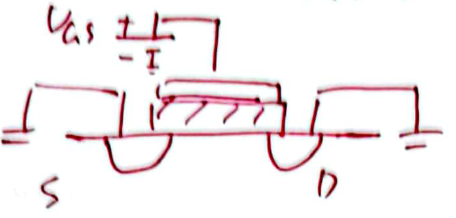
\includegraphics[scale=0.6]{1.jpg}
    \captionsetup{labelformat=empty}
    \caption{$V_{GS}>V_{TH}$, $V_D=V_S=0$}
    \label{1}
\end{figure}

MOSFET turned on, but has no current.

\subsection*{Case \uppercase\expandafter{\romannumeral2}: $V_{GS}>V_{TH}$, $V_D>V_S=0$}

\begin{figure}[htbp]
    \centering
    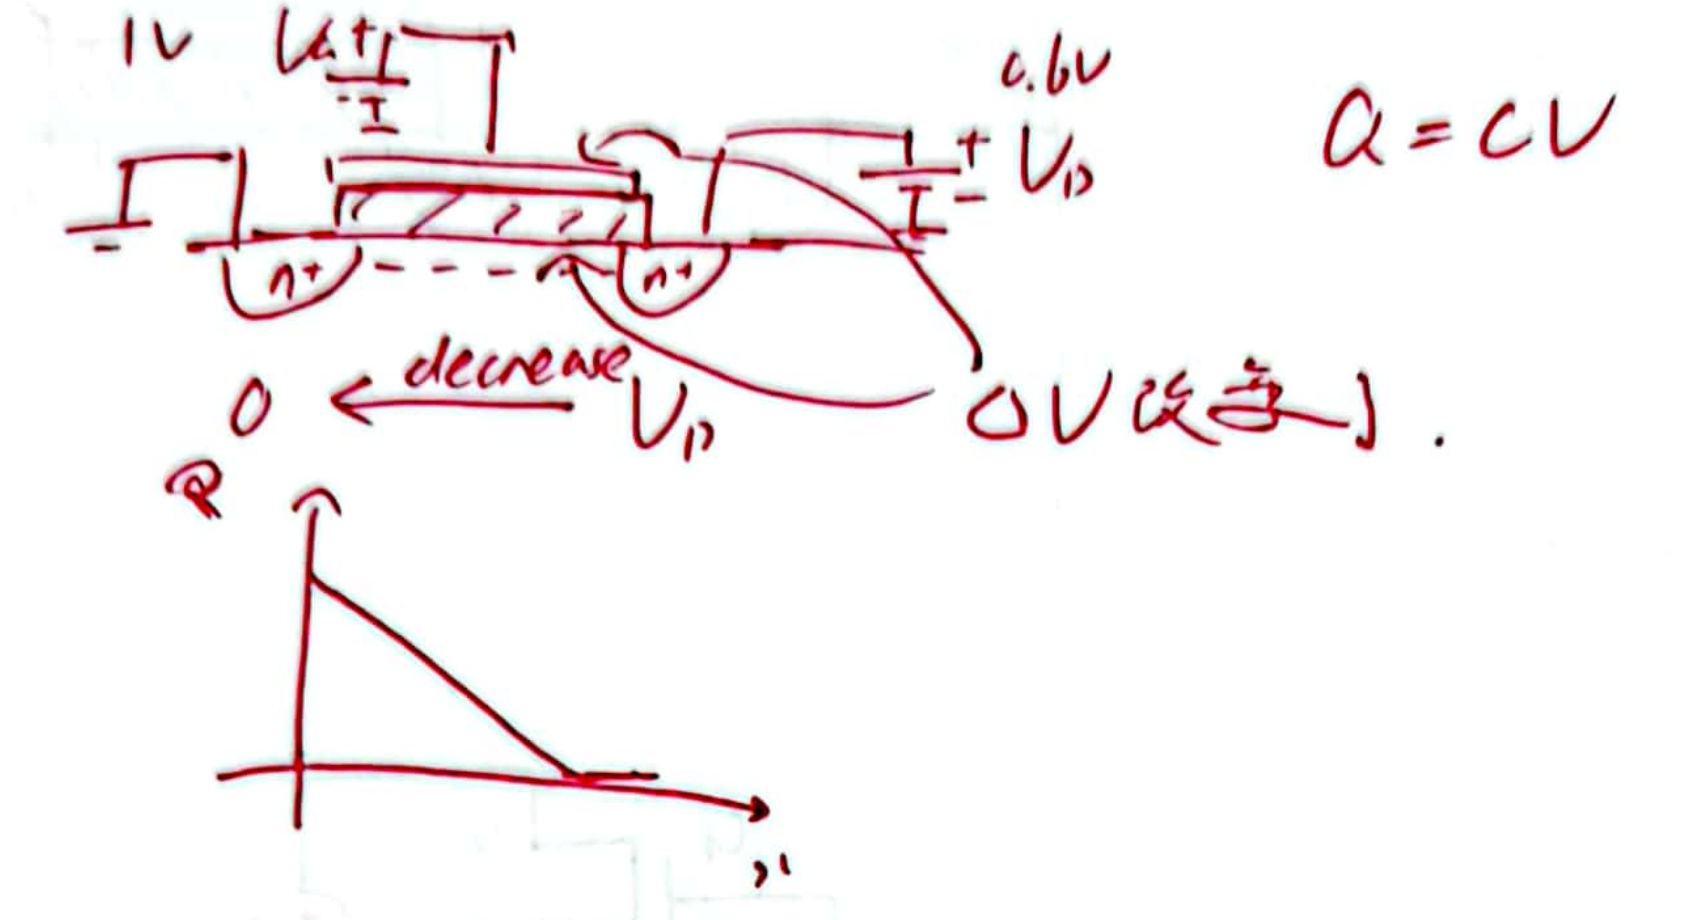
\includegraphics[scale=0.3]{2.jpg}
    \captionsetup{labelformat=empty}
    \caption{$V_{GS}>V_{TH}$, $V_D>V_S=0$}
    \label{2}
\end{figure}

When $V_D$ is applied, A voltage drop occurs between the S and D,
resulting in the voltage between the upper and lower plates not being equal to the $V_G$.
It decreases from the D to the S.

With $Q=CV$, we can draw a Q-X relationship diagram. That indicates $I_D$ is related to $V_{DS}$.

\section*{Dimensions of MOSFET}

\begin{figure}[htbp]
    \centering
    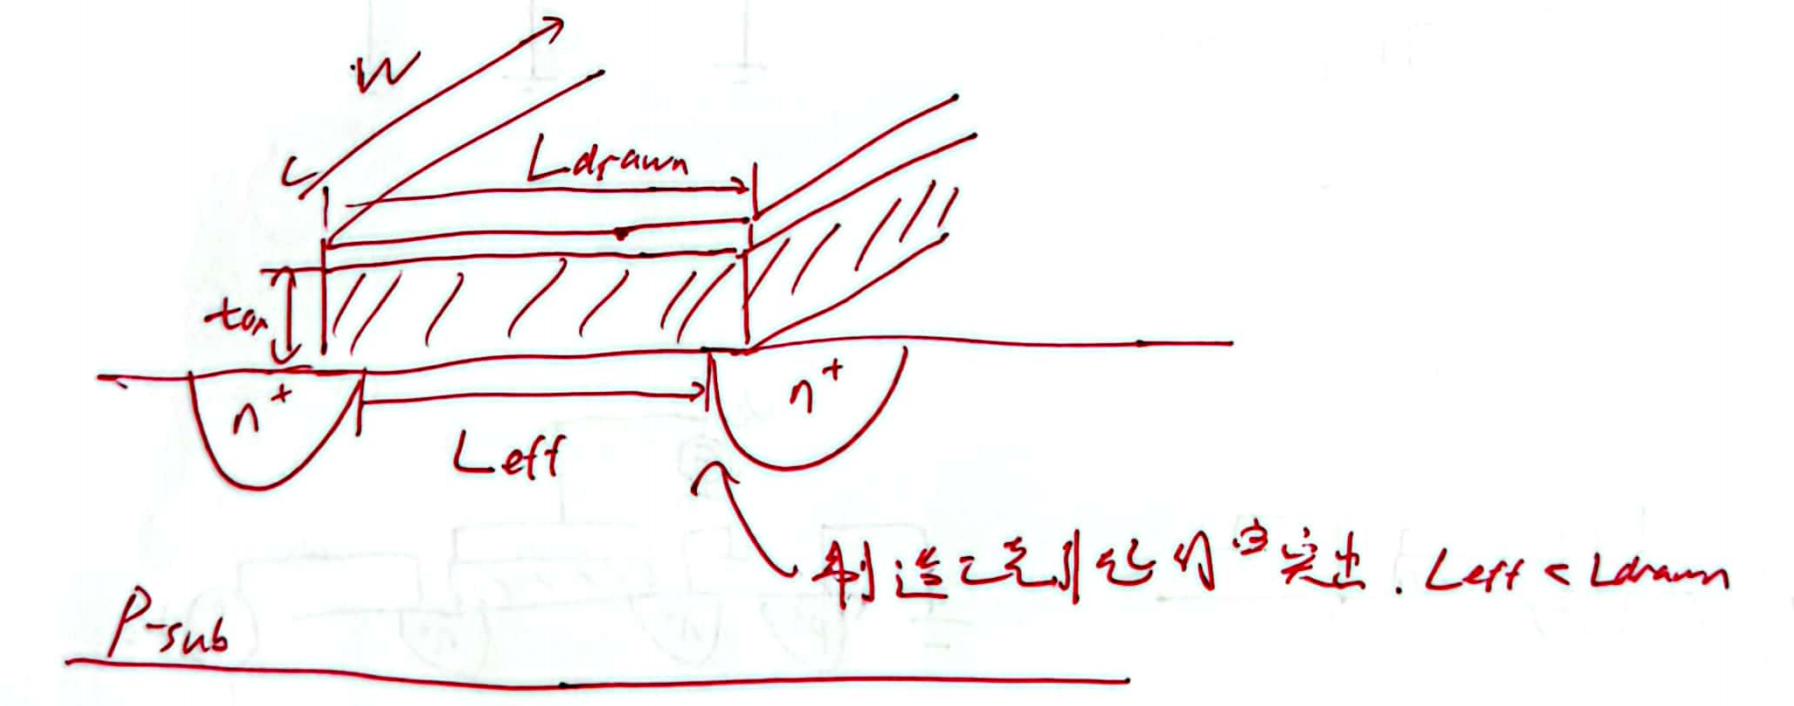
\includegraphics[scale=0.4]{3.jpg}
    \captionsetup{labelformat=empty}
    \caption{Dimensions of MOSFET}
    \label{3}
\end{figure}

Affected by the manufacturing process, the n-type semiconductor and silicon dioxide oxide layers at both ends overlap a little.
We call this length $L_{eff}$, and the length of the gate metal plate is called $L_{drawn}$.

\section*{Derivation of I/V Characteristic}

\subsection*{Channel Charge Density}

\subsubsection*{Case \uppercase\expandafter{\romannumeral1}: $V_{GS}>V_{TH}$, $V_D=V_S=0$}

$Q_{ch,total}=W*L_{eff}*C_{ox}*(V_{GS}-V_{TH})$

We call $V_{GS}-V_{TH}$ the overdrive voltage, $C_{ox}$ the capper of unit area.

$Q_{ch,density}=W*C_{ox}*(V_{GS}-V_{TH})$

\subsubsection*{Case \uppercase\expandafter{\romannumeral2}: $V_{GS}>V_{TH}$, $V_D>V_S=0$}

$Q_{ch,density}=W*C_{ox}*(V_{GS}-V_{TH}-V(x))$

V is x-dependence, see the Behavour of Channel's Case \uppercase\expandafter{\romannumeral2}.

\subsection*{Drain Current}

\begin{figure}[htbp]
    \centering
    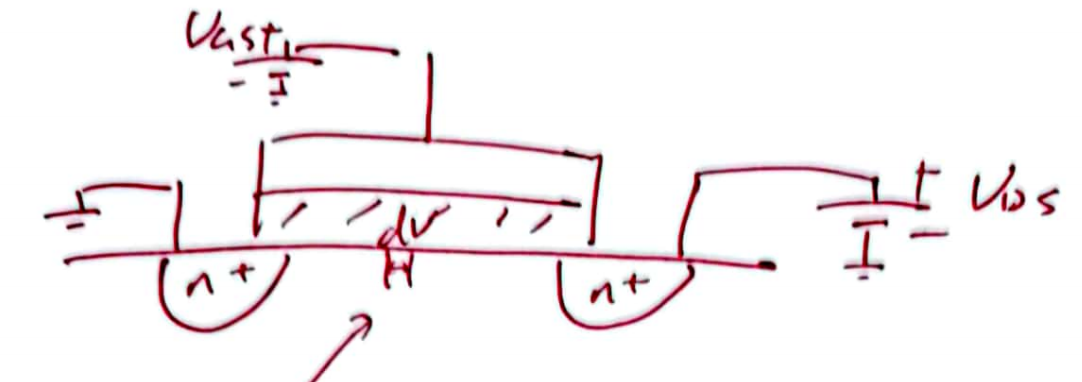
\includegraphics[scale=0.4]{4.jpg}
    \captionsetup{labelformat=empty}
    \caption{Calculate drain current}
    \label{4}
\end{figure}

We just mentioned that if a voltage is applied to the drain, a current will be generated.

We know that $v=\mu_{n}E$, $E=-\frac{dV}{dx}$.

So we get $v=-\mu_{n}\frac{dV}{dx}$.

From $Q_{ch,density}=W*C_{ox}*(V_{GS}-V_{TH}-V(x))$,

Select a unit length, we get

$$I_D=-v*Q_{ch,density}=-[-\mu_{n}\frac{dV}{dx}*W*C_{ox}*(V_{GS}-V_{TH}-V(x))]$$

Note that $I_D$ is a constant.

Move $dx$ to the left and integrate both sides of the equation, we get

$$\int_{0}^{L} I_Ddx=\mu_{n}*W*C_{ox}*\int_{0}^{V_{DS}} (V_{GS}-V_{TH}-V(x))dV$$

$L$ in these equations always refers to $L_eff$.

Simplify the equation, we get

$$I_D=\mu_{n}*C_{ox}*\frac{W}{L}[(V_{GS}-V_{TH})*V_{DS}-\frac{1}{2}V_{DS}^2]$$

Pay attention $V_{GS} \geq V_{TH}$ here.

Then we can get their relationship curves.

\begin{figure}[htbp]
    \centering
    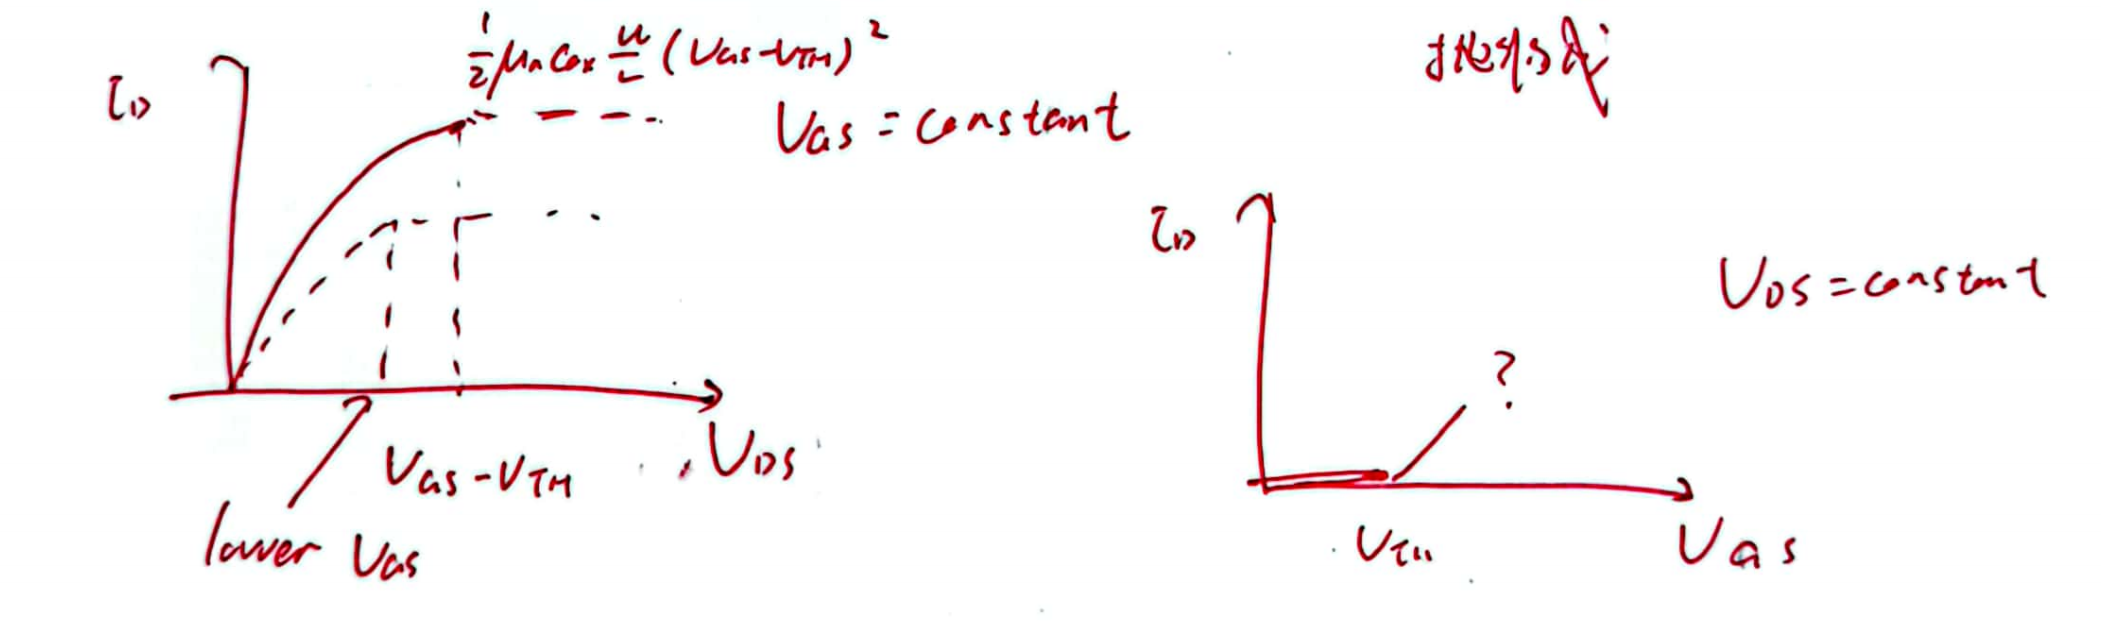
\includegraphics[scale=0.4]{5.jpg}
    \captionsetup{labelformat=empty}
    \caption{The relationship between $I_D$, $V_{DS}$ and $V_{GS}$}
    \label{5}
\end{figure}

Now we haven't known how the $I_D$ change if $V_{DS}>V_{GS}-V_{TH}$ or $V_{GS}$ increases.

\section*{Link}

\href{https://www.bilibili.com/video/BV1FD4y1R7Ah?p=30&vd_source=1d0c07486a3bd3b0adb8ac548bf6453e}{Razavi Electronics Circuits 1: lectrue 30}
\end{document}